%%%%%%%%%%%%%%%%%%%%%%%%%%%%%%%%%%%%%%%%%%%%%%%%%%%%%%%%%%%%%%%%%%%%%%%
%%%%%%%%%%%%%%%%%%%%%%%%%%%%%%%%%%%%%%%%%%%%%%%%%%%%%%%%%%%%%%%%%%%%%%%
\deelmetoef{Module 1}{Inleiding}{Module 1. Inleiding}{Oplossingen module 1}{Oplossingen module 1}
\label{sec:inl}
%%%%%%%%%%%%%%%%%%%%%%%%%%%%%%%%%%%%%%%%%%%%%%%%%%%%%%%%%%%%%%%%%%%%%%%
%%%%%%%%%%%%%%%%%%%%%%%%%%%%%%%%%%%%%%%%%%%%%%%%%%%%%%%%%%%%%%%%%%%%%%%

\begin{samenvatting}
Tijdens dit project maken we een smartphone app waarmee je je hartslag kan meten. Waarom het belangrijk is af en toe je hartslag te meten en waarom we dit met een app willen doen, wordt hierna uitgelegd. Daarna bekijken we wat een hartslag nu precies is, en hoe we die met onze smartphone kunnen meten.
\end{samenvatting}
%

%%%%%%%%%%%%%%%%%%%%%%%%%%%%%%%%%%%%%%%%%%%%%%%%%%%%%%%%%%%%%%%%%%%%%%%
\section{Wat en waarom?}
\label{sec:Mod1_Sec1}
%%%%%%%%%%%%%%%%%%%%%%%%%%%%%%%%%%%%%%%%%%%%%%%%%%%%%%%%%%%%%%%%%%%%%%%
%
De hartslag duidt aan hoe vaak je hart klopt per minuut. Tijdens het sporten is het belangrijk je hartslag in het oog te houden. Een te hoge hartslag wijst op een te hoge inspanning, en kan mogelijks gevaarlijk zijn. Bovendien kan een (te) hoge hartslag in rust wijzen op aandoeningen zoals een overactieve schildklier, bloedarmoede of bloedverlies, een longaandoening enz. Regelmatig je hartslag controleren is dus de boodschap.

Om je hartslag te meten wordt meestal gebruik gemaakt van een bloeddrukmeter.

\begin{minipage}{.5\linewidth}
	\gewonefiguur{width=\linewidth}{module1/patient}
\end{minipage} 
\begin{minipage}{.5\linewidth}
	\gewonefiguur{width=\linewidth}{module1/hartslagmonitor}
\end{minipage} 

Een bloeddrukmeter is een gespecialiseerd toestel dat meestal enkel een dokter of iemand met hartklachten ter beschikking heeft. Bovendien is het nogal omslachtig een bloeddrukmeter tijdens het sporten mee te nemen, gezien dit niet echt een draagbaar toestel is.

\gewonefiguur{width=.5\linewidth}{module1/lopermethartslagmeter}

Naast een bloeddrukmeter kan ook een hartslagmeter gebruikt worden om de hartslag te meten. 

\begin{minipage}{.5\linewidth}
	\gewonefiguur{width=\linewidth}{hartslagmeter}
\end{minipage} 
\begin{minipage}{.5\linewidth}
	\gewonefiguur{width=\linewidth}{module1/loper-met-dure-loopband}
\end{minipage} 

In tegenstelling tot een bloeddrukmeter kan je een hartslagmeter wel makkelijk meenemen bij het sporten. Bovendien geeft de hartslagmeter ook real time feedback; dat wil zeggen dat je op elk moment quasi onmiddellijk je hartslag zien. Maar wellicht ligt de aanschaf van een hartslagmeter niet binnen het budget van elke leerling of student?

Daarom bouwen wij in dit project onze eigen smartphone app, waarmee we snel, eenvoudig en redelijk accuraat onze hartslag kunnen meten, zonder nood aan gespecialiseerde toestellen.

\gewonefiguur{width=.5\linewidth}{module1/loper}

\section{De hartslag}
\label{sec:Mod1_Sec2}

Je hart is een spier, die samentrekt om je bloed in je lichaam rond te pompen. De hartslag is de pompbeweging van je hart. In de volksmond is de hartslag ook het aantal samentrekkingen van je hart per minuut, of anders gezegd het aantal keer dat je hart klopt per minuut.

De hartslag van een volwassene varieert tussen 60 en 100 slagen per minuut. De maximale hartslag (aangeduid als $MH$) is de hoogste hartslag die je lichaam aan kan gedurende fysische activiteit. De maximale hartslag varieert naargelang je leeftijd en kan berekend worden met de volgende vuistregel

\begin{equation*}
MH = 220-LT
\end{equation*}

met volgende notatie:
\begin{itemize}
	\item MH: maximale hartslag met als eenheid slagen per minuut of \textquotedblleft beats per minute \textquotedblright (kortweg: \emph{bpm}). 
	Dit noteren we als MH [bpm].
	\item LT [jaar]: leeftijd
\end{itemize}

Het wordt aangeraden tijdens het sporten je hartslag tussen 55 en 85\% van je maximale hartslag te houden. 

Voor een volwassene van 20 jaar oud is het aangeraden hartslagbereik tijdens het sporten dus tussen 110 en 170 bpm.
Voor een volwassene van 50 jaar oud is het aangeraden hartslagbereik tijdens het sporten lager, nl. tussen 97 en 145 bpm.

\begin{table}
	\centering
	\begin{tabular}{c|ccc}
		LT & MH & 0,55*MH & 0,85*MH \\
		\hline
		20 & 200 & 110 & 170 \\
		50 & 170 & 94 & 145 
	\end{tabular}
\end{table}

\begin{oef}
Bereken de maximale hartslag $MH$ en het ideale hartslagbereik tijdens het sporten van een volwassene van 
\begin{itemize}
	\item 18 jaar
	\item 30 jaar
	\item 65 jaar
\end{itemize}
\end{oef}
\oplos{\begin{itemize}
		\item $MH_{18}=202$ en hartslagbereik tussen 111,1 en 171,7
		\item $MH_{30}=190$ en hartslagbereik tussen 104,5 en 161,5
		\item $MH_{65}=155$ en hartslagbereik tussen 85,25 en 131,75
	\end{itemize}
}

\begin{oef}Maak ook een grafiek die de maximale hartslag $MH$ uitzet in functie van de leeftijd $LT$. 

Welke grootheid komt op de $x$-as? Wat is de eenheid? 

Welke grootheid komt op de $y$-as? Wat is de eenheid?
\end{oef}
\oplos{
	\begin{tikzpicture}[domain=0:100]
	\begin{axis}[axis lines=middle,xmax=110,ymin=-1,ymax=240,
		x label style={at={(axis description cs:0.5,-0.1)},anchor=north},
		y label style={at={(axis description cs:-0.1,.5)},rotate=90,anchor=south},
		xlabel={LT (Jaar)},ylabel={MH (bpm)}]
	\addplot[domain=0:100] {220-x} node[left]{$MH=220-LT$};
	\end{axis}
	\end{tikzpicture}
}

De hartslag, of het rondpompen van je bloed, voel je als je je hand op je hart legt. Maar ook in je hals of aan je pols kan je je hartslag voelen. De hartslag wordt dan ook vaak handmatig gemeten door twee gestrekte vingers op de pols (van jezelf of van een ander persoon) of in de hals (tegen de halsslagader) te plaatsen. Hier voel je de hartslag heel goed. Door gedurende 15 seconden het aantal hartslagen te tellen en te vermenigvuldigen met vier kan je de hartslag, dit is het aantal keer dat je hart pompt per minuut of per 60 seconden, bepalen.

\begin{opdracht}{Opdracht: Je eigen hartslag meten}
	Meet je eigen hartslag door twee gestrekte vingers in je hals te plaatsen, het aantal keer dat je hart pompt gedurende 15 seconden te tellen en dit te getal te vermenigvuldigen met vier.
	
	Als je moeite hebt om het aantal hartslagen te tellen, kan je ook gebruik maken van de smartphone app \textquoteleft Science journal\textquoteright. De app kan je downloaden in de Google Play Store.\footnote{Tip voor leerkachten:
	Het gebruik van de app Science Journal kan je demonstreren door je smartphone scherm te projecteren op je computer. Hiervoor kan je het programma (op je pc) en de app (op je smartphone) Vysor gebruiken wanneer je smartphone met een USB kabel met de pc verbonden is.}
	
	Start een nieuw experiment en meet het omgevingsgeluid, zoals in de figuur hieronder. Plaats twee gestrekte vingers in je hals en zeg \textquoteleft ja\textquoteright \ elke keer als je een hartslag voelt. Doe dit gedurende 15 seconden. Tel nadien het aantal pieken dat geregistreerd werd en vermenigvuldig dit aantal met vier om de hartslag te bekomen.
	
	\begin{minipage}{.5\linewidth}
		\figuurmetlabel[\label{fig:app_scienceJournal}]{height=12cm}{module1/illustratieScienceJournal}{De app Science journal. Gebruik de luidspreker om je stem en het omgevingsgeluid op te nemen.}
	\end{minipage}
	\begin{minipage}{.5\linewidth}
		\figuurmetlabel[\label{fig:meting_scienceJournal}]{height=12cm}{module1/metingScienceJournal}{Voorbeeld van een geluidsmeting in Science Journal. \newline}
	\end{minipage}

	Zo tellen we voor bovenstaande meting 15 pieken op 15 seconden. De hartslag bekomen we door dit aantal te vermenigvuldigen met vier: de hartslag is 60 bpm.

\end{opdracht}

\begin{oef}
	Met welke factor moet je het aantal hartslagen gemeten gedurende een telperiode van 10 seconden vermenigvuldigen om de hartslag in \emph{bpm} te bekomen? 
	
	En wat als de telperiode 20 seconden is?
	
	Wat is het voordeel van een langere telperiode?
\end{oef}
\oplos{\begin{itemize}
		\item $10~s$: factor $6$
		\item $20~s$: factor $3$
		\item Hoe korter de telperiode, hoe nauwkeuriger je moet tellen. Eventuele telfouten worden immers vermenigvuldigd met de factor. De factor is groter, naarmate de telperiode korter is. Telfouten worden dus groter als de telperiode korter is.
	\end{itemize}
}

Voor heel hoge hartslagen ($>160~bpm$) wordt het quasi onmogelijk de hartslag nog zelf te tellen. Dan moet je een meettoestel gebruiken. In wat volgt maken wij ons eigen meettoestel: een smartphone app waarmee je goedkoop, snel en gemakkelijk je hartslag kan meten.

\section{Overzicht van het project}
\label{sec:Mod1_Sec3}

Maar hoe kunnen we met onze smartphone onze hartslag gaan meten? We hebben al gezien dat je het pompen van je hart goed kan voelen aan je pols of in de hals. Net zo is de hartslag ook waarneembaar in je vingertop; ook daar zijn kleine pulsaties in je aders door het pompen van je hart. 

\gewonefiguur{height=10cm}{module1/loperStilstaand}

We zullen gebruik maken van de camera die in je smartphone ingebouwd is. We zullen onze vingertop zachtjes op de lens van de camera plaatsen. De kleine pulsaties in de aders van je vinger resulteren in kleine veranderingen in de kleur van je vinger. Met het blote oog kan je die miniscule kleurveranderingen niet waarnemen, maar gelukkig kan je die subtiele veranderingen wel met je smartphone detecteren. De kleurveranderingen in functie van de tijd zijn gerelateerd aan het pompen van je hart. Een grafiek van de kleurverandering in functie van de tijd zie je hieronder. Door opnieuw het aantal pieken in de telperiode van 15 seconden te tellen en te vermenigvuldigen met vier bekom je opnieuw de hartslag.

%TODO figuur maken en invoegen (Excel?)

De opeenvolging van uit te voeren stappen kunnen we voorstellen in een blokdiagram, zoals hieronder. Dit blokdiagram toont welke stappen we moeten doorlopen om de hartslag te bepalen, zonder in detail uit te werken wat precies moet gebeuren in elk blok. Dit laat ons toe een bondig overzicht te geven van het project, zonder dat we nu al precies moeten weten wat in elke stap moet gebeuren.

We willen de kleurwaarde van je vingertop in functie van de tijd analyseren. 
De kleurwaarde van je vingertop wordt geregistreerd met de camera van je smartphone en opgeslaan als een filmpje.
Een video of een filmpje is in feite niet meer dan een aantal foto's die heel snel na elkaar getoond worden op een scherm.
Die foto's laten ons toe om te bepalen wat de kleurwaarde van je vingertop was op het moment dat de foto werd genomen.
We hebben drie verschillende manieren om vanuit die kleurwaarden de hartslag te bepalen.
Ten eerste, als we de kleurwaarde van alle foto's op die verschillende tijdstippen achter elkaar zetten in een grafiek, zien we een aantal pieken zoals hieronder. 
Daaruit kunnen we zelf berekenen wat onze hartslag was op het moment dat het filmpje werd opgenomen, door zoals voordien het aantal pieken te tellen en te vermenigvuldigen met een factor om het aantal pieken per minuut te bekomen.
Ten tweede kunnen we de smartphone ook automatisch die pieken laten herkennen, het aantal pieken laten tellen en dit aantal herleiden naar het aantal pieken per minuut.
Dit bespaart ons heel wat rekenwerk.
Ten derde bestaat er nog een andere methode, met een Fouriertransformatie die op complexere wiskunde gebaseerd is, die ons toelaat de hartslag te bepalen. 
Vooral wanneer de meting een beetje ruizig is, wanneer als we de pieken moeilijk kunnen herkennen, zal deze methode nauwkeuriger zijn.
Hoe deze methode concreet werkt, wordt uitgelegd in Sectie \ref{sec:piekdetectie}.

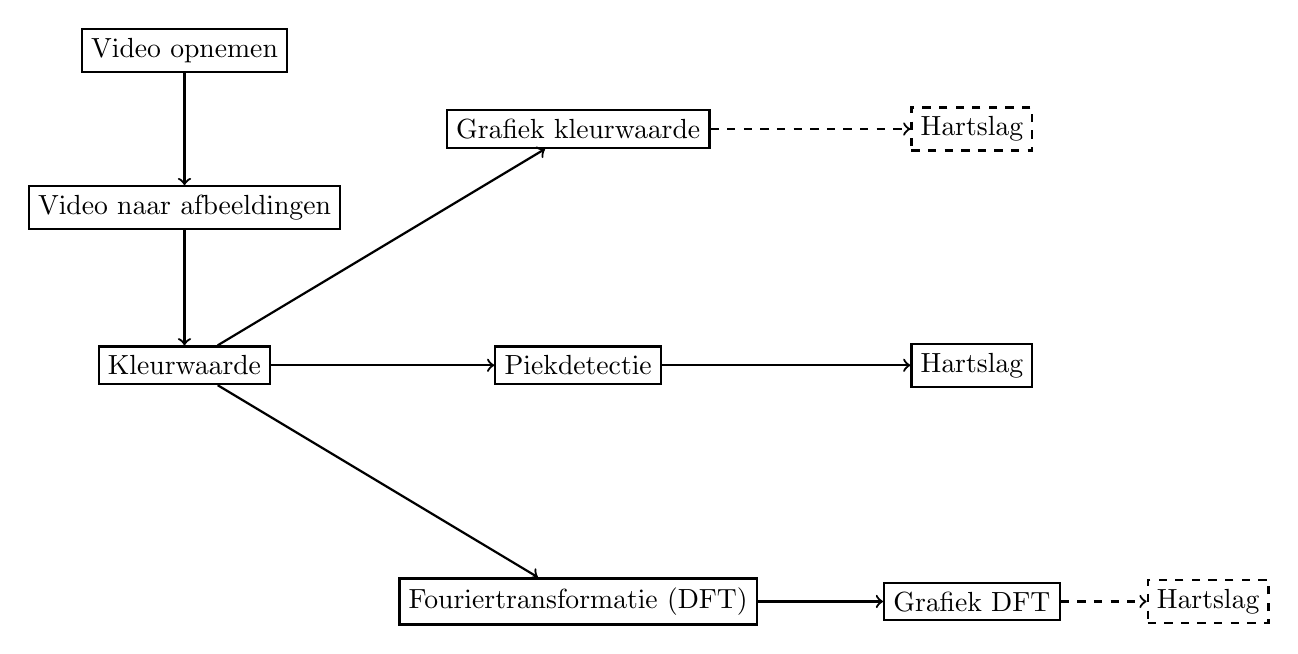
\begin{tikzpicture}[thick]
\node[draw,rectangle] at (0,0) (a) {Video opnemen};
\node[draw,rectangle] at (0,-2) (b) {Video naar afbeeldingen};
\node[draw,rectangle] at (0,-4) (c) {Kleurwaarde};
\node[draw,rectangle] at (5,-1) (d) {Grafiek kleurwaarde};
\node[draw,rectangle,dashed] at (10,-1) (j) {Hartslag};
\node[draw,rectangle] at (5,-4) (e) {Piekdetectie};
\node[draw,rectangle] at (10,-4) (f) {Hartslag};
\node[draw,rectangle] at (5,-7) (g) {Fouriertransformatie (DFT)};
\node[draw,rectangle] at (10,-7) (h) {Grafiek DFT};
\node[draw,rectangle,dashed] at (13,-7) (i) {Hartslag};

\draw[->] (a) -- (b) ;
\draw[->] (b) -- (c) ;

\draw[->] (c) -- (d) ;
\draw[->] (c) -- (e) ;
\draw[->] (c) -- (g) ;

\draw[->,dashed] (d) -- (j) ;
\draw[->] (e) -- (f) ;
\draw[->] (g) -- (h) ;
\draw[->,dashed] (h) -- (i) ;

\end{tikzpicture}

%\begin{tikzpicture}
%\sbEntree{n1}
%\sbRelier[RecordButton]{n1}
%\sbBlocL{n1}{Video opnemen}{n2}
%%\sbBlocL{n2}{Video naar afbeeldingen}{n3}
%%\sbBlocL{n3}{Kleurwaarde van afbeeldingen}{n4}
%%\sbBlocL{n4}{Grafiek van kleurwaarde ifv tijd}{n5}
%%\sbBlocL{n5}{Piekdetectie kleurwaarden}{}
%%\sbBlocL{n6}{Hartslag berekenen}{n7}
%%\sbSortie[5]{S1}{n7}
%%\sbNomLien[0.8]{S1}{$Hartslag$}
%
%%\sbEntree{E}
%%\sbComp{a}{E}
%%\sbBloc{b}{$H_1$}{a}
%%\sbRelier[$E_1$]{E}{a}
%%\sbBlocL{c}{$H_2$}{b}
%%\sbRelier[$\epsilon$]{a}{b}
%%\sbComph{d}{c}
%%\sbRelier[u]{c}{d}
%%\sbBlocL{e}{$H_3$}{d}
%%\sbBlocL{f}{$H_4$}{e}
%%\sbSortie[5]{S1}{f}
%%\sbRelier{f}{S1}
%%\sbNomLien[0.8]{S1}{$S_1$}
%%\sbDecaleNoeudy[-4]{f}{u}
%%\sbDecaleNoeudy{e}{v}
%%\sbBlocr{r1}{$R_1$}{u}
%%\sbBlocr{r2}{$R_2$}{v}
%%\sbBlocrL{r3}{$R_3$}{r2}
%%\sbRelieryx{f-S1}{r1}
%%\sbRelierxy[n1]{r1}{d}
%%\sbRelieryx{e-f}{r2}
%%\sbRelierxy[n2]{r3}{a}
%\end{tikzpicture}




